\chapter{测试与评估}\label{chap:eval}

本章围绕 QuickBoard 的核心目标进行测试与评估，重点验证：弱网与断线条件下的最终收敛、对象规模增长下的渲染性能，以及高频过程预览链路的网络降载效果。

\section{测试策略}
项目采用“单元测试 + 构建验证 + 可复核实验”的组合策略：
\begin{itemize}
  \item \textbf{单元测试}：覆盖协作通信、OCR 请求与裁剪、同步逻辑等核心模块，降低迭代带来的回归风险。
  \item \textbf{构建验证}：确保生产构建通过，避免仅开发环境可运行的问题。
  \item \textbf{可复核实验}：以一致性对照实验、渲染性能基准与降载统计测试对关键结论进行量化验证，并形成报告归档。
\end{itemize}

\section{单元测试与构建结果}
前端使用 Vitest 执行单元测试，并在每轮关键改动后执行构建验证。测试与构建输出以报告形式归档在 \texttt{doc/test\_reports}，便于回溯与论文撰写引用。

\begin{table}[htbp]
  \centering
  \caption{工程验证项汇总}\label{tab:verification}
  \renewcommand{\arraystretch}{1.35}
  \begin{tabular}{lll}
    \toprule
    \textbf{验证项} & \textbf{目的} & \textbf{结果} \\
    \midrule
    前端单元测试 & 覆盖核心逻辑、降低回归 & 通过 \\
    前端生产构建 & 确保可交付与可部署 & 通过 \\
    OCR 识别链路自检 & 验证预处理与返回格式 & 通过 \\
    \bottomrule
  \end{tabular}
\end{table}

\section{一致性对照实验：朴素广播 vs.\ LWW+补包}
为了验证弱网与断线场景下的最终收敛，采用 6 个客户端参与对照实验，并在接收侧引入丢包、延迟与抖动，同时对部分客户端施加断线窗口。评价指标选取“结束时哈希种类数”：对每个客户端结束时的权威对象集合做稳定序列化并计算哈希，统计不同哈希的数量。若系统最终一致，则哈希种类数应为 1；若出现分叉，则大于 1。

\begin{table}[htbp]
  \centering
  \caption{一致性对照实验关键结果}\label{tab:sync-benchmark}
  \renewcommand{\arraystretch}{1.35}
  \begin{tabular}{llll}
    \toprule
    \textbf{方案} & \textbf{网络扰动} & \textbf{断线窗口} & \textbf{结束时哈希种类数} \\
    \midrule
    朴素广播（naive） & recv drop=0.15, delay=90ms, jitter=140ms & clients=1,2 断线 2400ms & 6 \\
    LWW+补包（lww） & recv drop=0.15, delay=90ms, jitter=140ms & clients=1,2 断线 2400ms & 1 \\
    \bottomrule
  \end{tabular}
\end{table}

实验结果表明，朴素广播在丢包与断线条件下容易产生多版本分叉；采用服务端权威裁决、字段级 LWW 与版本补包后，系统能够收敛到单一权威状态。

\subsection{指标适用性讨论}
“结束时哈希种类数”用于回答“最终是否收敛到同一对象集合”这一问题，其优点是计算简单、可复核且不依赖主观判断。该指标的局限在于无法刻画收敛过程中的短时不一致程度，也无法表达意图保持等更强语义。考虑到 QuickBoard 的目标是短会话协作下的最终可用与可对齐，本章选择该指标与研究目标一致；若进一步研究意图保持或离线合并，则需要引入更细粒度的评估维度与数据结构支持。

\section{渲染性能基准：视口裁剪与对象缓存}
渲染基准在 6000$\times$6000 世界坐标内生成 5000 个对象，对比 Baseline（\texttt{skipOffscreen=false}, \texttt{objectCaching=false}）与 Optimized（\texttt{skipOffscreen=true}, \texttt{objectCaching=true}）两组配置，采样统计平均渲染耗时。基准结果来自项目归档报告。

\begin{table}[htbp]
  \centering
  \caption{渲染性能基准关键结果}\label{tab:render-benchmark}
  \renewcommand{\arraystretch}{1.35}
  \begin{tabular}{llll}
    \toprule
    \textbf{场景} & \textbf{Baseline avg render(ms)} & \textbf{Optimized avg render(ms)} & \textbf{可见对象占比} \\
    \midrule
    idle & 57.500 & 26.950 & $\approx 2.8\%$ \\
    pan & 52.275 & 16.225 & $\approx 2.8\%$ \\
    \bottomrule
  \end{tabular}
\end{table}

结果显示，在大对象规模场景下，视口裁剪显著降低参与绘制的对象数量；配合对象缓存可进一步降低重复绘制开销，从而明显降低平均渲染耗时。

\section{过程预览降载：Ghost Brush 统计验证}
过程预览属于高频瞬时数据，若逐点发送容易造成消息风暴并挤占权威增量带宽。针对 Ghost Brush 预览链路，采用算法级统计测试进行验证：10s 内以 4ms 采样（理论 2500 点），通过批处理与限包策略统计实际消息数。

\begin{table}[htbp]
  \centering
  \caption{Ghost Brush 降载测试关键结果}\label{tab:ghost-brush}
  \renewcommand{\arraystretch}{1.35}
  \begin{tabular}{llll}
    \toprule
    \textbf{采样点数（理论）} & \textbf{实际消息数} & \textbf{降载倍率} & \textbf{isEnd 次数} \\
    \midrule
    2500 & 279 & 8.96$\times$ & 1 \\
    \bottomrule
  \end{tabular}
\end{table}

统计结果表明，在保证轨迹连续展示与结束信号正确的前提下，批处理与限包机制能显著降低预览链路的消息数量，有助于降低多人同时书写时的网络压力。

\section{弱网实验入口示例}
图 \ref{fig:netsim} 展示了基于 URL 参数启用弱网扰动后的画板页面示例，用于说明实验条件可控。

\begin{figure}[htbp]
  \centering
  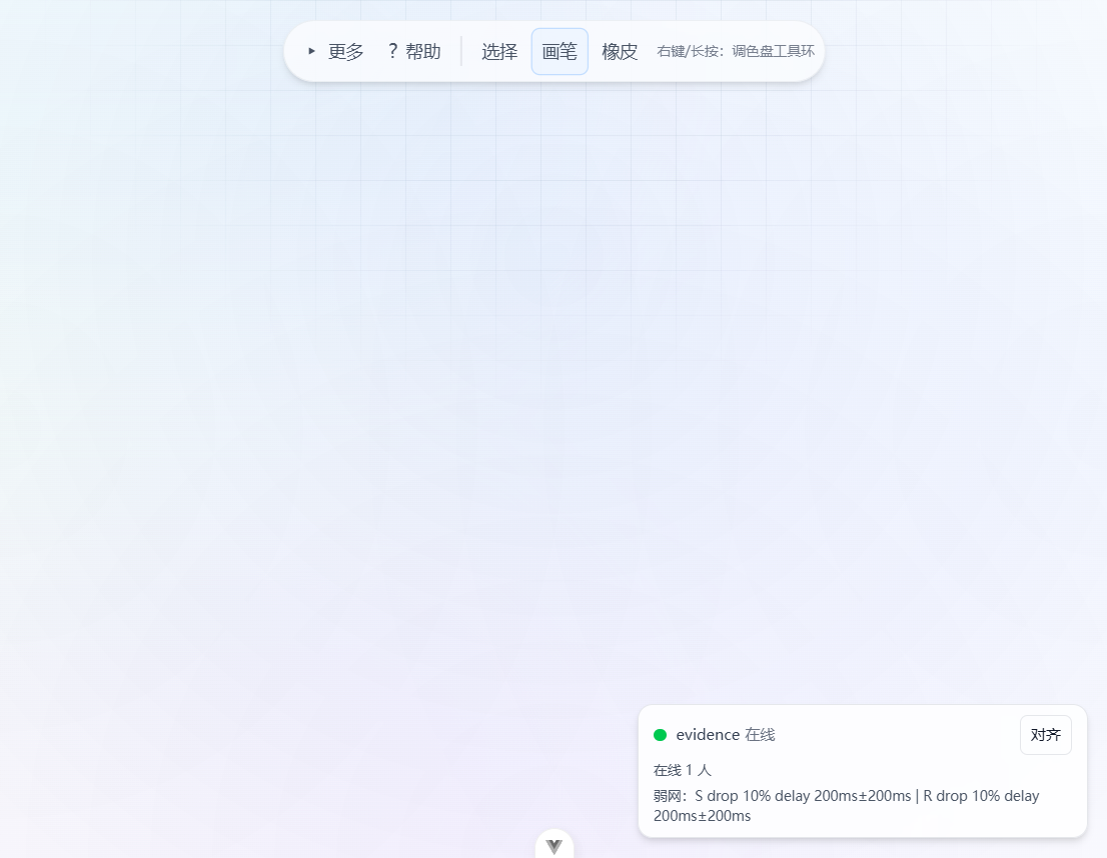
\includegraphics[width=0.92\linewidth]{figures/S3_netsim.png}
  \caption{弱网扰动参数开启示例}\label{fig:netsim}
\end{figure}

\section{威胁与局限性}
本课题的评估主要依赖工程脚本与自动化报告，能够保证可复核，但仍存在局限性：
\begin{itemize}
  \item \textbf{弱网扰动覆盖范围}：弱网模拟通过参数化丢包、延迟与抖动来构造网络扰动，无法完全覆盖真实移动网络中的复杂行为（例如链路层重传、突发拥塞与多路径切换）。
  \item \textbf{一致性语义范围}：字段级 LWW 强调最终收敛与实现可解释性，在极端并发同字段编辑时可能出现意图覆盖；本章指标侧重最终是否收敛，未对意图保持做进一步量化评估。
  \item \textbf{OCR 评估范围}：OCR 识别质量受输入分布与模型能力影响较大，本文强调可定位与可纠错的工程闭环，但未构建大规模数据集进行统计学评估。
\end{itemize}

\section{本章小结}
本章围绕 QuickBoard 的核心贡献给出三类可复核证据：一致性对照实验用于验证弱网与断线条件下的最终收敛；渲染基准用于量化对象规模增长下的性能改善；降载测试用于验证过程预览链路的消息量显著下降，并解释其对权威同步带宽的保护作用。通过将工程实现与评估证据绑定，论文论证从“实现了什么”进一步落到“为何有效、如何验证”。

\section{结果分析与不足}
从评估结果看，QuickBoard 的一致性策略在弱网与断线条件下能够实现最终收敛；渲染优化策略能够在对象规模较大时降低平均渲染耗时；过程预览降载能够显著降低消息量并减少对权威增量的干扰。其不足主要体现在：字段级 LWW 在极端并发同字段编辑时存在意图覆盖的语义取舍；OCR 识别质量仍受输入质量与场景分布影响；Canvas 渲染与对象模型在更大规模对象下仍可能出现性能瓶颈，后续可进一步探索更细粒度的渲染分层或 WebGL 路径。
